%%%%%%%%%%%%%%%%%%%%%%%%%%%%%%%%%%%%%%%%%
% FRI Data Science_report LaTeX Template
% Version 1.0 (28/1/2020)
%
% Jure Demšar (jure.demsar@fri.uni-lj.si)
%
% Based on MicromouseSymp article template by:
% Mathias Legrand (legrand.mathias@gmail.com)
% With extensive modifications by:
% Antonio Valente (antonio.luis.valente@gmail.com)
%
% License:
% CC BY-NC-SA 3.0 (http://creativecommons.org/licenses/by-nc-sa/3.0/)
%
%%%%%%%%%%%%%%%%%%%%%%%%%%%%%%%%%%%%%%%%%


%----------------------------------------------------------------------------------------
%	PACKAGES AND OTHER DOCUMENT CONFIGURATIONS
%----------------------------------------------------------------------------------------
\documentclass[fleqn,moreauthors,10pt]{ds_report}
\usepackage[english]{babel}

\graphicspath{{figures/}}




%----------------------------------------------------------------------------------------
%	ARTICLE INFORMATION
%----------------------------------------------------------------------------------------

% Header
\JournalInfo{UL FRI - Biomedical signal and image processing}

% Type of report
\Archive{Assigment 3 Report}

% Article title
\PaperTitle{Analysis of computed tomography (CT) images using Canny edge detector}

% Authors and their info
\Authors{Aljaz Mur Erzen\textsuperscript{1}}
\affiliation{\textsuperscript{1}\textit{ae4664@student.uni-lj.si, 63160011}}

% Keywords
\Keywords{hearbeat, detection, signal}
\newcommand{\keywordname}{Keywords}


%----------------------------------------------------------------------------------------
%	ABSTRACT
%----------------------------------------------------------------------------------------

%----------------------------------------------------------------------------------------

\begin{document}

% Makes all text pages the same height
\flushbottom

% Print the title and abstract box
\maketitle

% Removes page numbering from the first page
\thispagestyle{empty}

%----------------------------------------------------------------------------------------
%	ARTICLE CONTENTS
%----------------------------------------------------------------------------------------

\section*{Introduction}
	
Automatic analysis of computed tomography (CT) images plays a key role in assistance to medical experts in finding abnormalities and predicting possible diseases. As the first step in the pipeline, edge detection heavily contributes to reliability and performance of the whole analysis system.

This report describes internal mechanisms of Canny edge detection and our implementation for detection on CT images.

%------------------------------------------------

\section*{Blurring and derivation}

An edge can be thought of as a sharp transition from one segment of similar color to another. If our gray scale image would be a smooth, continuous function of x and y, we could compute directional derivatives and simply threshold them to find areas considered as an edge.

Directional derivative is related to rate of change of a function in the given direction. Or more geometrically: the angle quotient of a tangent line to our function in given point and direction.

Fortunately, there is no need for derivatives in \textit{all} directions, but only the two that are parallel to the x-axis and y-axis. These are called partial derivatives. When one or both of them have high absolute value, we know that there is high rate of change in \textit{some} direction, therefore we have encountered an edge.

Unfortunately, input images are not continuous and contain noise which prevents us from easily computing derivatives. Instead we could compute differentials, which are just subtraction between adjacent pixels. This subtraction can be represented by convolution with vector $\begin{bmatrix}-1, 1\end{bmatrix}$. It would not, however, solve the problems with noise so instead of using just two adjacent pixels, we apply convolution with larger vector of similar, but smoother shape: derivative of gaussian function (DoG). Size of the vector representing its discretized form is determined by parameter of the gaussian function: $\sigma$.

\begin{figure}[h]\centering
	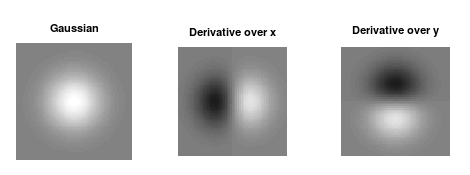
\includegraphics[width=\linewidth]{gaussians.png}
	\caption{\textbf{Gaussian and its derivatives over x and y}}
	\label{fig:gaussians}
\end{figure}

Note that DoG can be decomposed into convolution of one dimensional gaussian with one dimensional derivative of gaussian. This allows us to apply two smaller convolutions instead of one large, improving computational complexity:
\begin{equation}
	\begin{aligned}
		\frac{\partial I}{\partial x} \approx I_x 
		& = I \ast \frac{\partial G}{\partial x} 
		= I \ast (\frac{\partial g}{\partial t}^T \ast g)
		= (I \ast \frac{\partial g}{\partial t}^T) \ast g\\
		\frac{\partial I}{\partial y} \approx I_y 
		& = I \ast \frac{\partial G}{\partial x} 
		= I \ast (\frac{\partial g}{\partial t} \ast g^T)
		= (I \ast \frac{\partial g}{\partial t}) \ast g^T\\
	\end{aligned}
\end{equation}

For the subsequent steps, will need only the magnitude (2-norm of the partial derivatives) and their directions: 

\begin{equation}
	\begin{aligned}
		I_{mag}(x, y) & = |\begin{bmatrix}I_x(x, y) \\ I_y(x, y)\end{bmatrix}|_2 
			= \sqrt{I_x^2(x, y) + I_y^2(x, y)} \\
		I_{dir}(x, y) & = \arctan(I_y(x, y) / I_x(x, y))
	\end{aligned}
\end{equation}

\begin{figure*}[h]\centering
	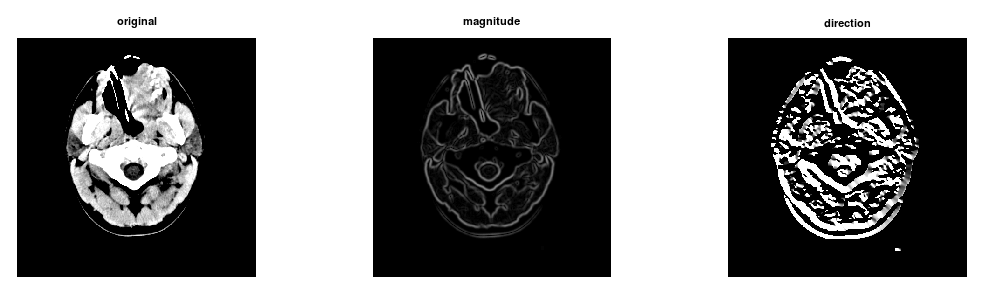
\includegraphics[width=\linewidth]{mag_dir.png}
	\caption{\textbf{Derivation of CT scan} Magnitude is a great edge indicator, but it still has to be thinned and binarized to become useful for further pipeline processing.}
	\label{fig:gaussians}
\end{figure*}

\section*{Non-maximum suppression}

Gradient is defined as a vector of partial derivatives over all input variables (x and y in our case). Its direction in a given point is aligned with direction of greatest descent. If the given point represents an edge, the gradient vector will be parallel to the edge.

This is useful for non-maximum suppression, a method of line thinning which takes the partial derivative magnitude image and removes (sets to zero) all pixels that are not local maximums in direction of the gradient. In effect, it should thin an edge in direction parallel to the edge. 

Our implementation solves this by simple comparisons of magnitude values in the correct direction. Due to discrete image coordinates, we cannot take into account all possible directions, which is why we discretize the gradient direction into 4 angles with the following formula: 
\begin{equation}
	\alpha = round((I_{dir} + \pi \mod \pi) / \pi * 4) \mod 4	
\end{equation}

\begin{figure}[h]\centering
	
\includegraphics[width=0.4\linewidth]{angle.png}
	\caption{\textbf{Discretization of direction to 4 classes} The result of applying the "direction discretization function" for every possible gradient direction.}
	\label{fig:angle}
\end{figure}

Now we can simply compare the magnitude value to the neighboring pixels in one of the 4 discretized angles. The result can be seen in figure \ref{fig:local_max}.

\begin{figure}[h]\centering
	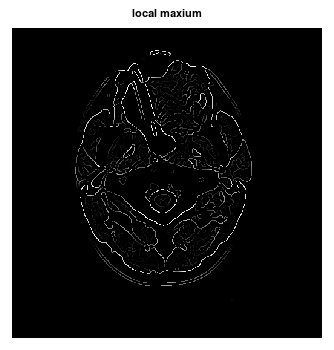
\includegraphics[width=0.7\linewidth]{local_max.png}
	\caption{\textbf{Non-maximum suppression}}
	\label{fig:local_max}
\end{figure}

\section*{Hysteresis threshold}

Simply applying a threshold to the magnitude image produces an image with may disconnected edges. To prevent this, we apply double threshold. All pixels whose magnitude is higher as the high threshold $t_{high}$ are marked as strong edges. All pixels that are not strong but whose magnitude is higher that the low threshold $t_{low}$ are marked as weak edges. 

The output image should contain all strong edges and those weak edges that are connected to some strong edge via 8 connectivity rule. We achieve this by first labeling each of the connected segments of weak or strong pixels. Then we pick all labels that contain at least one strong pixel and use all associated segments as the output image.

\begin{figure}[h]\centering
	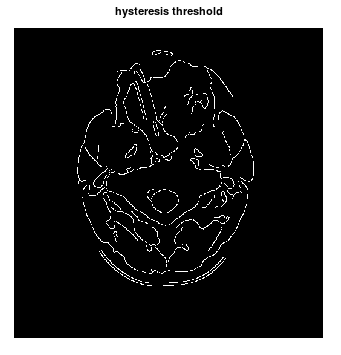
\includegraphics[width=0.7\linewidth]{threshold.png}
	\caption{\textbf{Hysteresis threshold}}
	\label{fig:threshold}
\end{figure}

This is considered the output of the Canny detector. But because the results of our implementation were very segmented, we decided to add another step.

\newpage

\section*{Edge linking}

The edges are now very disconnected, which is why we apply two simple morphological operations: dilation and erosion. Both of them take binary image as an input and output.

Dilation is a sliding-widow operator, where result of each window evaluation is computed as \texttt{OR} between all window pixels. Effectivity, all positive areas (our edges) in input get expanded (dilated), hence the name. 

Erosion is similarly a sliding-widow operator, but the result of each window evaluation is computed as \texttt{AND} between all input pixels. Effectivity, all positive areas (our edges) in input get shrunk (eroded). 

If we apply dilation and subsequent erosion, small gaps between edges may get filled during dilation but would not get eroded, thus connecting the gaps. The downside is that some smaller "holes" will also get filled-in, but for our application, this does represent a problem.

\section*{Results}

For the given input images, we have set the parameters empirically. It must be noted that the gaussian's $\sigma$ is highly dependent on image resolution, which in turn affects the two thresholds.

We have tested the algorithm on 6 images from the CTMRI database \cite{ctmri}.

\vspace{1em}\noindent
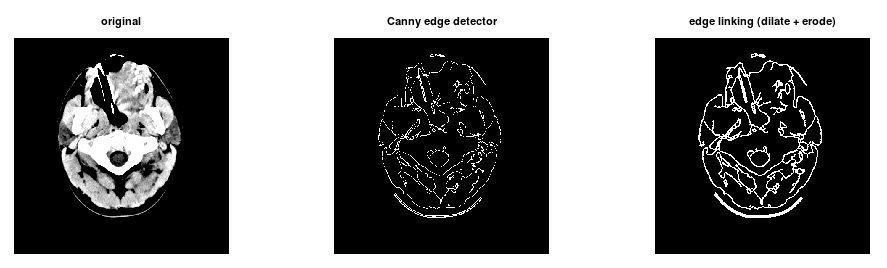
\includegraphics[width=\linewidth]{001.png}
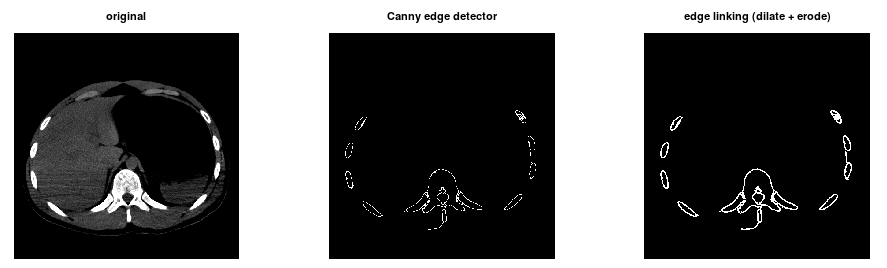
\includegraphics[width=\linewidth]{002.png}
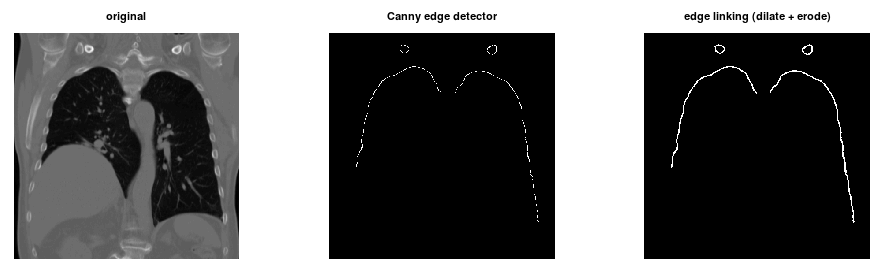
\includegraphics[width=\linewidth]{003.png}

\newpage\noindent
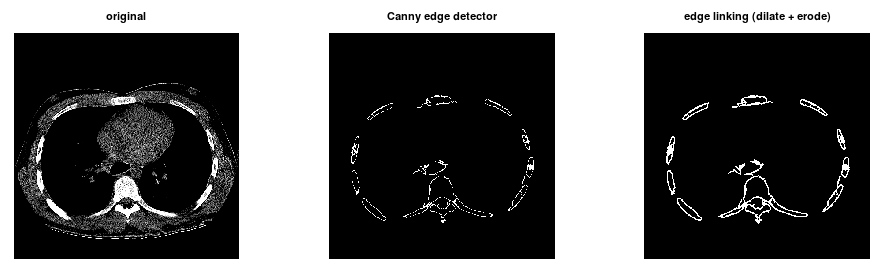
\includegraphics[width=\linewidth]{004.png}
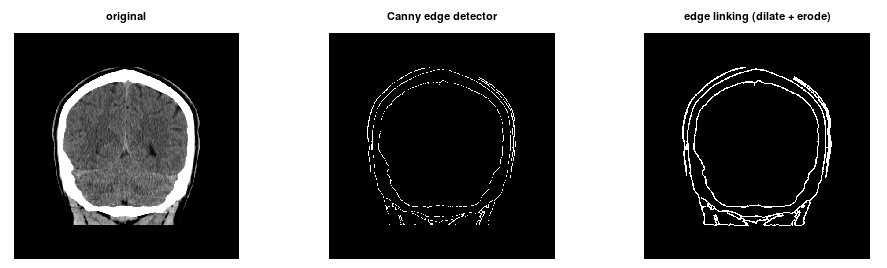
\includegraphics[width=\linewidth]{005.png}
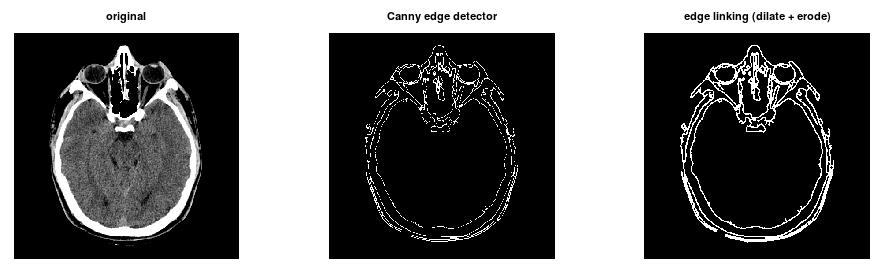
\includegraphics[width=\linewidth]{006.png}

\vspace{2em}
This relativity simple approach already produces useful results for further analysis processing.

The main pitfall of the current implementation seems to be simplification of non-maximum suppression. The discrete angles cause gaps within the edges which in turn highly degrades hysteresis thresholds which depend on segment connectivity. Angle discretization could be prevented by sub-pixel extrapolation to determine local maximums, which could be done without major computational complexity increase.

\bibliographystyle{unsrt}
\bibliography{report}


\end{document}
